\documentclass[letterpaper]{article}
\usepackage[utf8]{inputenc}
%\usepackage[ansinew]{inputenc}
\usepackage[spanish]{babel}
\usepackage{graphicx}

\begin{document}

\title{Proyecto 3\\ Laboratorio de Microcontroladores ADCs y Puerto Serial}
\author{
 Marco Antonio Montero Chavarría Carné: A94000\\
  \and
  Francisco Molina Carné: B14194\\  
}
\maketitle

\section{Cambios en la solución propuesta}
Para elaborar el graficador de señales efectivamente se implementó el esquema planeado de la figura \ref{diag1}, para ello lo primero que se trabajó fueron los bloques CDC ACM y ADC junto con la aplicación Minicom en linux para probar que efectivamente habiía comunicación serial entre el stm32 y la computadora. Posteriormente se elaboró un pequeño programa en python de prueba para recibir con pyserial los mismo datos pero en nuestra propia aplicación. \\[0.2 cm]

\begin{figure}[hbtp]
\centering
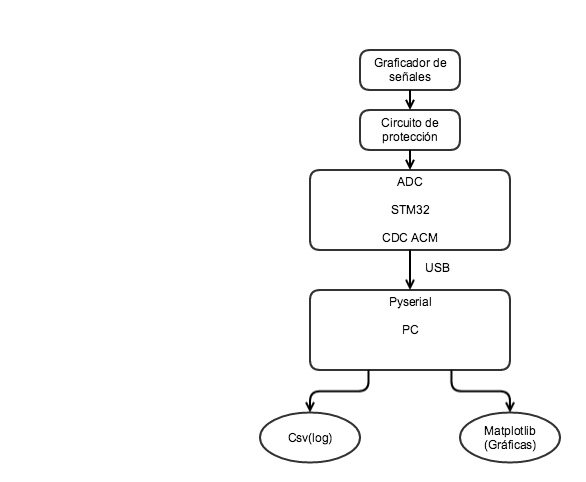
\includegraphics[width=8 cm]{flowdiag.png}
\caption{Esquema}
\label{diag1}
\end{figure}

\newpage

Una vez probado que se recibían los datos se pasó a montar el circuito de la figura \ref{circ1} como protección para el microcontrolador dando como resultado el circuito de la figura \ref{circ2}, donde encontramos el MCP6022 y resistencias de 680$\Omega$ y $470\Omega$ para realizar el divisor de tensiones de forma que la tensión que llega a la salida $V_o$ es igual a $V_o = \frac{470}{680} \cdot V_i = 0,69 V_i$ con lo que el máximo $V_i=5$ daría un $V_o=3,45$, sin embargo al tomar medidas con el multímetro, la entrada máxima del $V_i$ era de aproximadamente 4,3 con lo que la salida máxima del $V_o$ alcanzaba los 2,97 V. \\[0.2 cm]

\begin{figure}[hbtp]
\centering
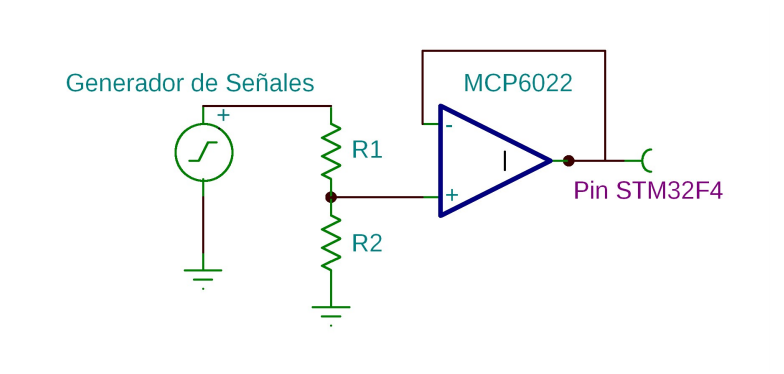
\includegraphics[width=8 cm]{circ1.png}
\caption{Circuito de protección}
\label{circ1}
\end{figure}
\begin{figure}[hbtp]
\centering
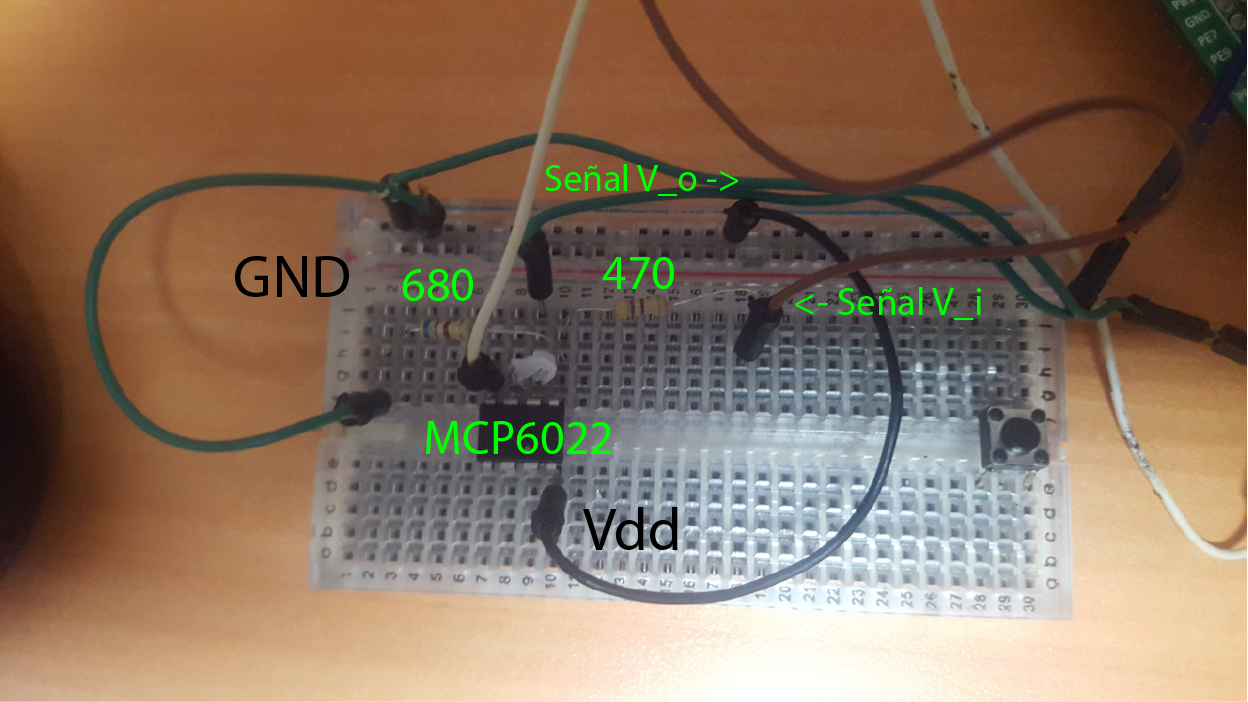
\includegraphics[width=8 cm]{circr.png}
\caption{Circuito de protección}
\label{circ2}
\end{figure}

\newpage

Ya con la tensión máxima asegurada por debajo de 3 V. se procedió a usar el graficador de matplotlib, junto con los datos recibidos de pyserial y con csv para guardar el log con los datos tomados. Como primera prueba se utilizó el código del archivo transmi2.py mostrado en la figura  \ref{t2} junto con el generador de ondas, lo que devolvió como resultado la figura  \ref{dat1} al muestrear claramente a más del doble de la frecuencia de la onda. 

\begin{figure}[hbtp]
\centering
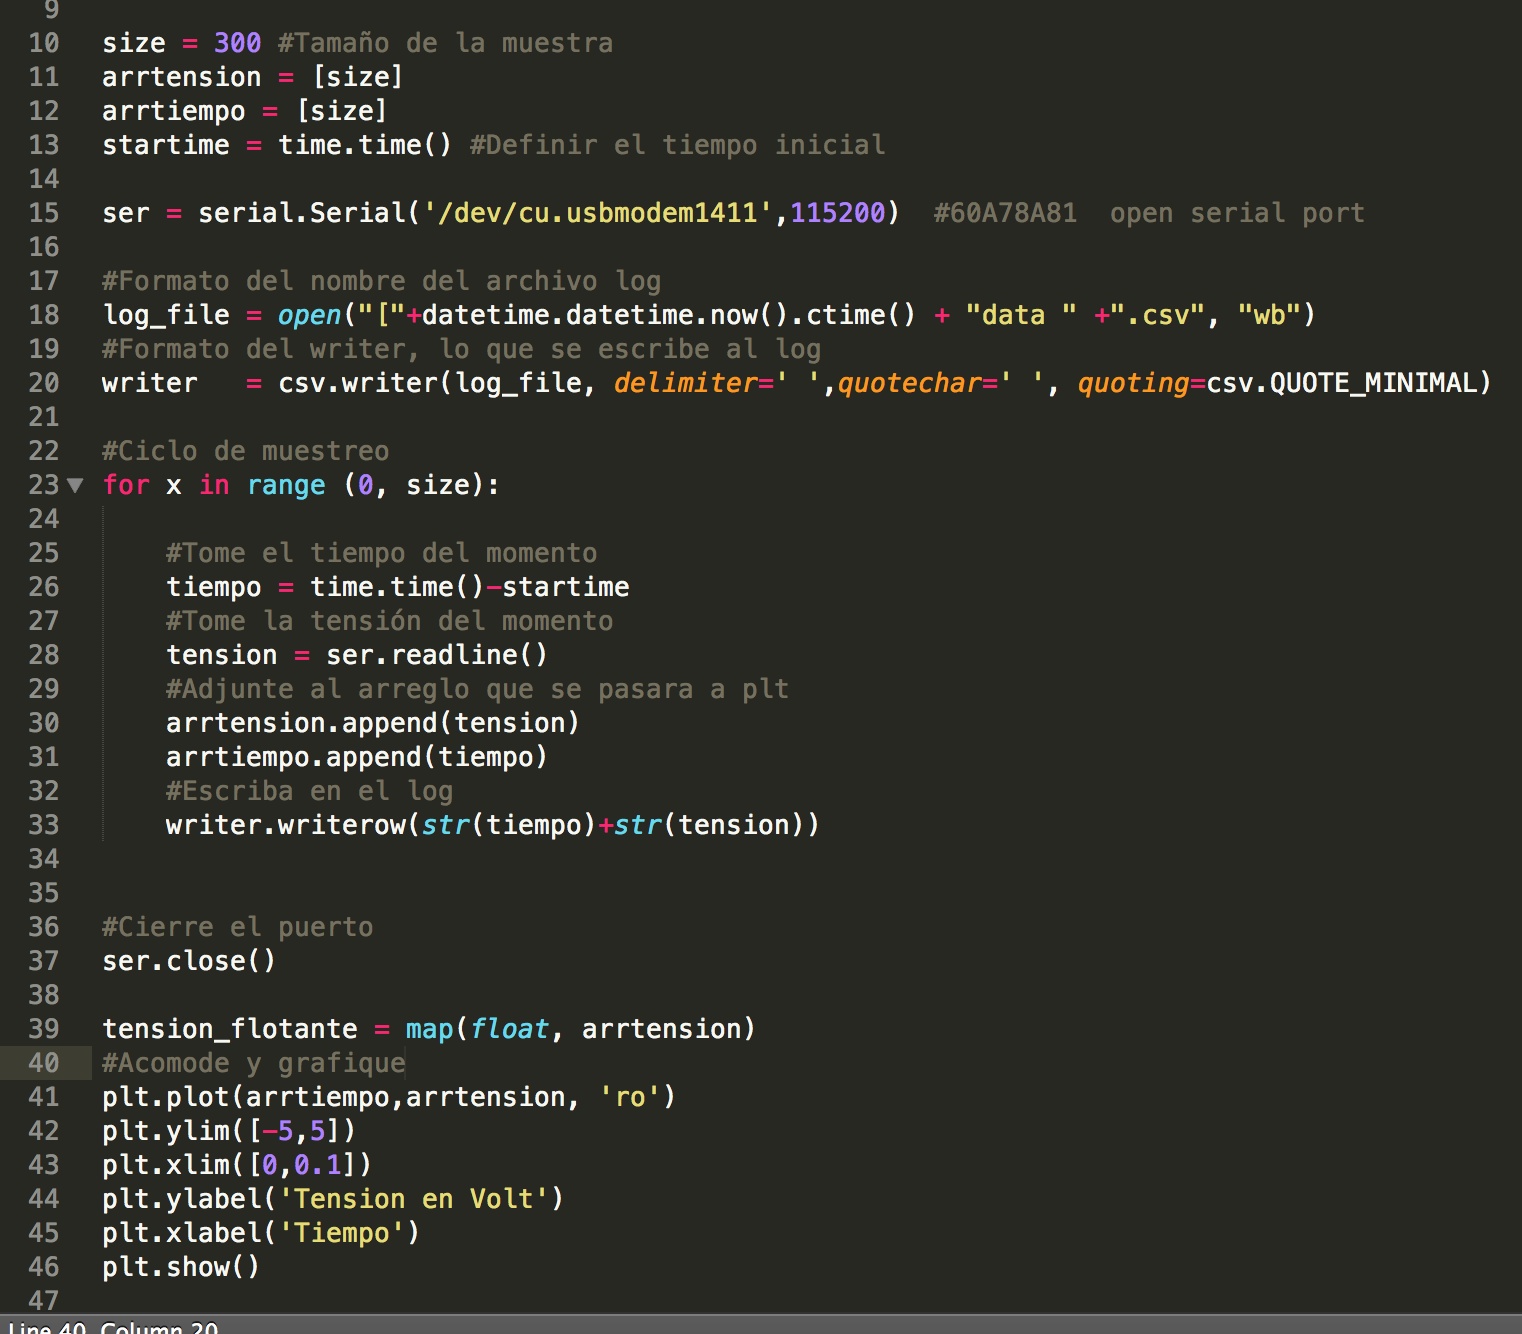
\includegraphics[width=12 cm]{normal.png}
\caption{Graficación normal}
\label{t2}
\end{figure}

\begin{figure}[hbtp]
\centering
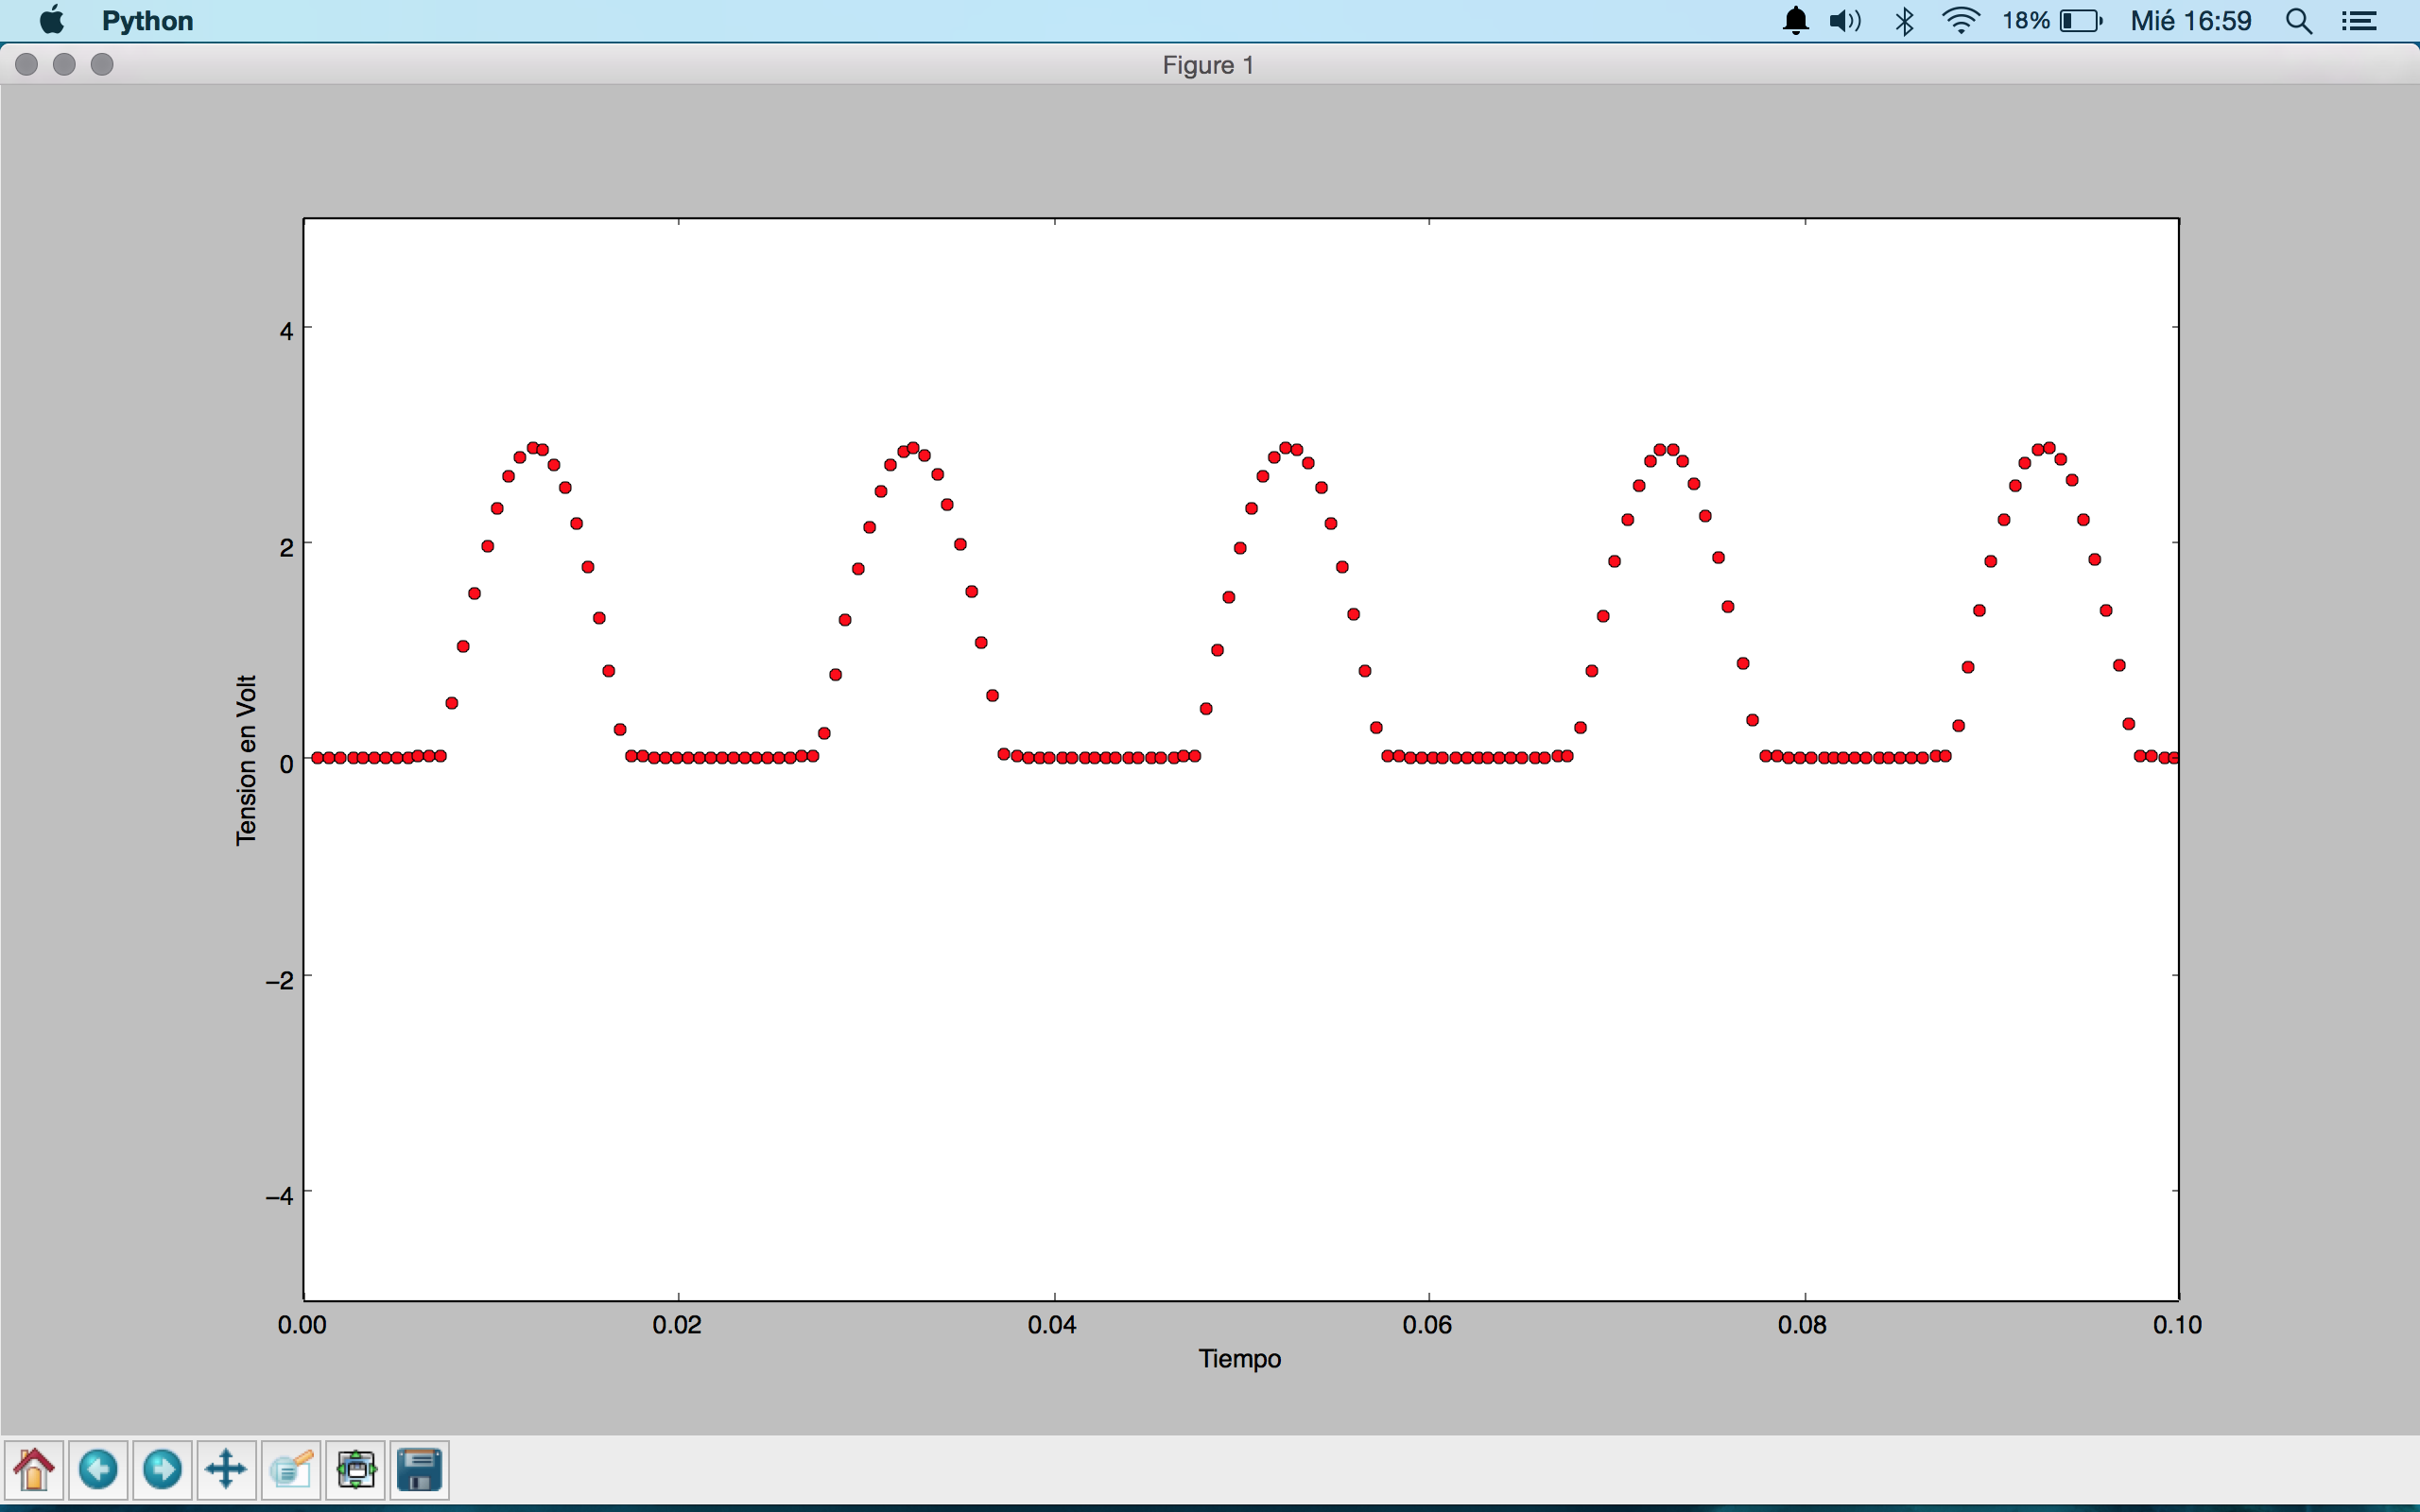
\includegraphics[width=12 cm]{signals.png}
\caption{Onda senoidal}
\label{dat1}
\end{figure}

\newpage

\section{Innovación}

Como innovación del proyecto se implementaron 2 mejoras, la primera fue utilizar un sensor de tacto externo mostrado en la figura \ref{touch}para verificar que se puede muestrear señales de cualquier periférico siempre y cuando se haga la conversión necesaria. La segunda fue implementar un código para muestrear en tiempo real los datos, de forma que se obtenga la señal en pantalla conforme se van tomando los datos.
El código del archivo transmi.py para esto lo podemos encontrar en la figura \ref{dat2} mientras que el sistema funcionando lo podemos encontrar en el video: https://youtu.be/9R3dfunGKa4 

\begin{figure}[hbtp]
\centering
\includegraphics[width=4 cm]{touch.png}
\caption{Sensor}
\label{touch}
\end{figure}

\begin{figure}[hbtp]
\centering
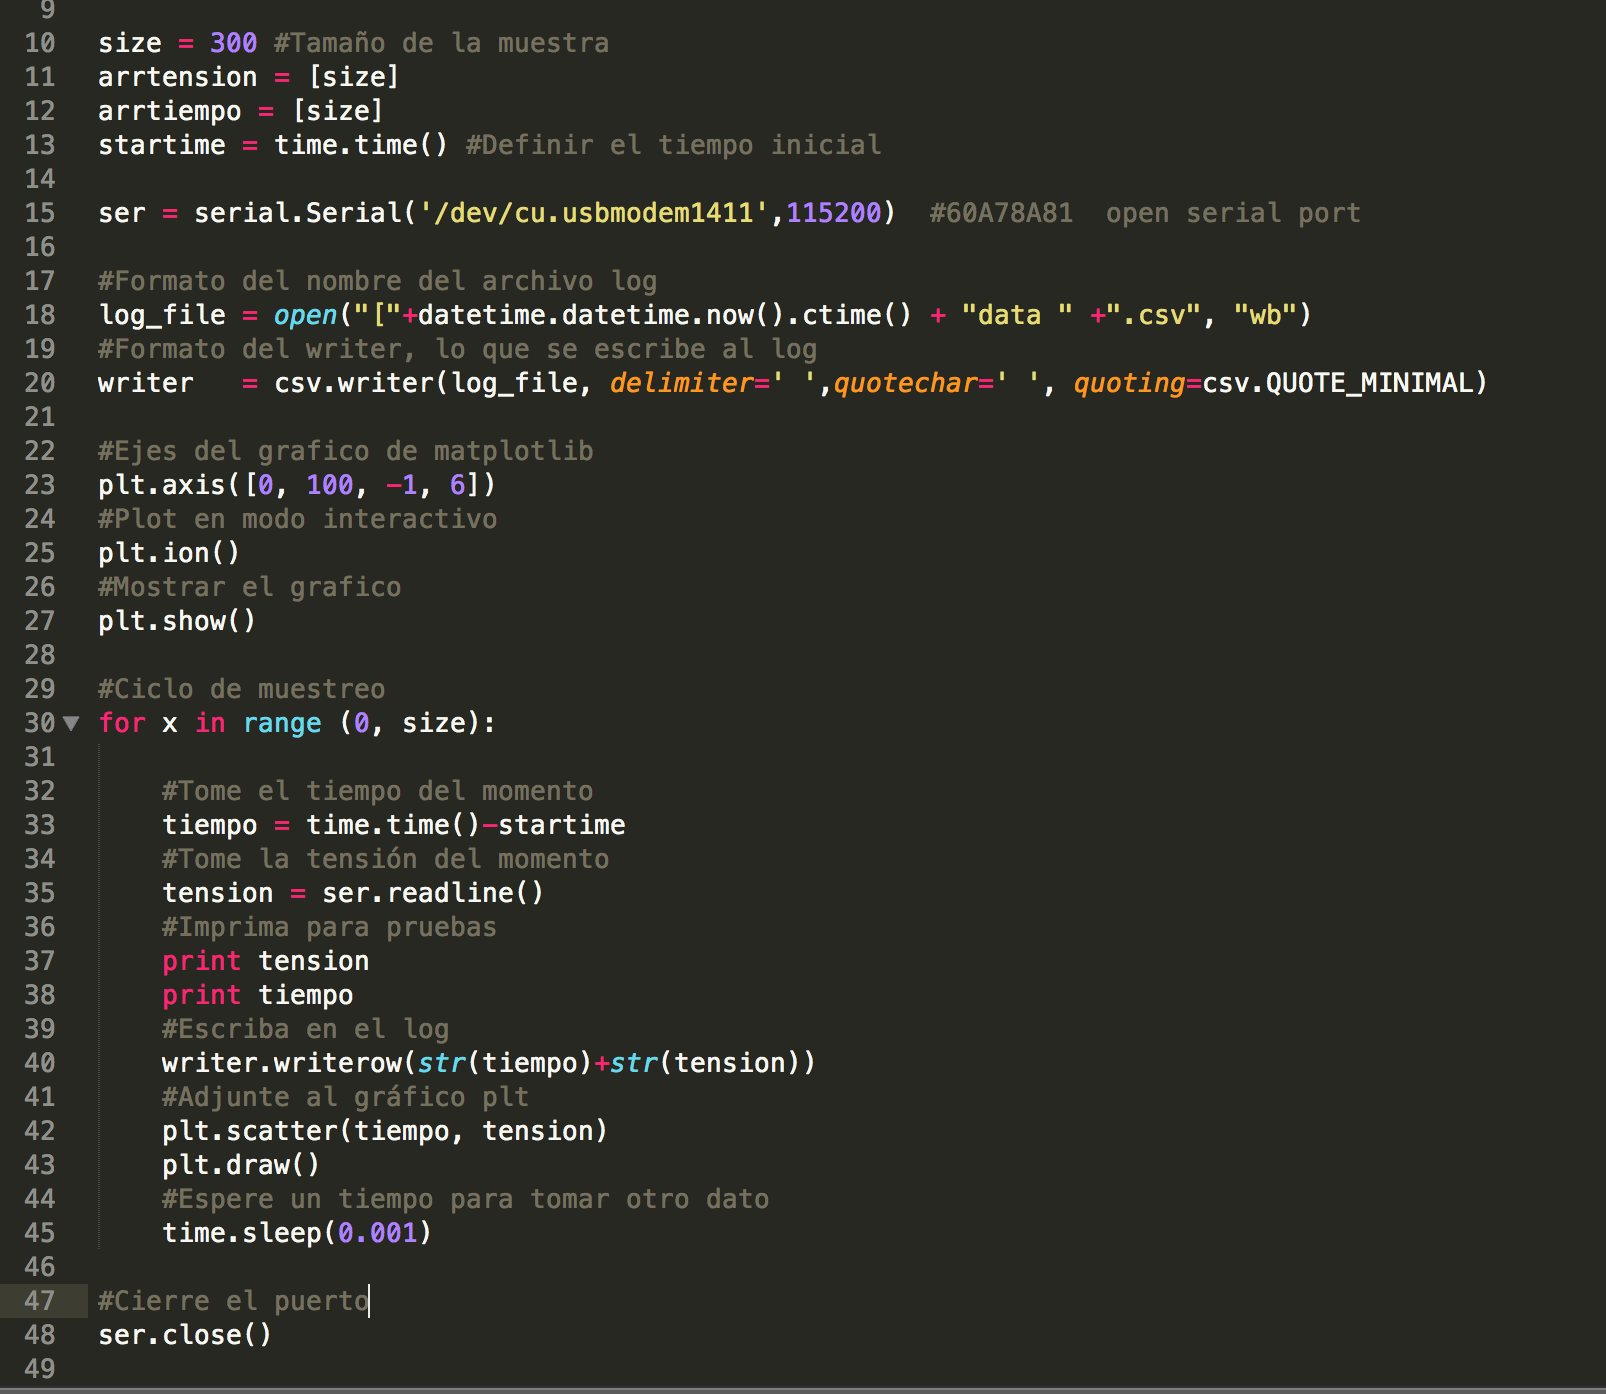
\includegraphics[width=12 cm]{tmpreal.png}
\caption{Tiempo real}
\label{dat2}
\end{figure}

\newpage
\section{Justificación de resultados}
El hecho de ir realizando poco a poco los diferentes pasos, y atacando los errores uno por uno sirvió para que el proyecto fuera realizado con éxito, en cuanto a las señales y la graficación en la primera parte se obtuvo lo deseado, sin embargo no se realizó la conversión de vualta a la escala 0V-5V, pero esto queda en recomendaciones para futuros proyectos, ya que es simplemente multiplicar el valor final. En cuanto a tiempos, solo hizo falta preocuparse por el tiempo de muestreo ya que los datos se tomaban y posteriormente se imprimian.\\[0.2 cm]
Para la parte de innovación, especialmente en la sección de graficación en tiempo real, la temporización fue muy importante, ya que se notó un apilamiento de los datos en por parte de la librería pyserial que se resolvió bajando la frecuencia de muestreo del STM para sincronizar la toma de datos con el muestreo, sin embargo lo preferible sería que el STM tome los datos y que el muestreo sea independiente de la frecuencia del STM. Por ello se hace referencia en las recomendaciones, verificar la temporizacion y el apilamiento de pyserial como el ciclo de atención a interrupciones del contador del STM.\\[0.2 cm]
En conclusión se lograron los objetivos del proyecto y se exploró un poco más los alcances tanto de las librerías como del microcontrolador, esto nos acerca al objetivo del proyecto final de forma que muestrear señales de un potenciómetro es realizable para el controlador que queremos elaborar.

\newpage
\section{Recomendaciones}

\begin{itemize}
\item En el caso de graficación en tiempo real, verificar los tiempos de muestreo del script en python y las frecuencias de trabajo del STM para la atención a interrupciones.
\item Agregar el multiplicador a la salida del archivo .py para recuperar la señal original.
\item Verificar la toma de datos y no el apilamiento, explorar las funcionalidades de pyserial.
\item Tener sumo cuidado con el circuito de protección, probar que las tensiones sean las adecuadas antes de conectarlo al STM, así como revisar los pines que se están utilizando.
\item Realizar pequeñas pruebas antes de programar cada parte y descomponer el problema en problemas más sencillos.
\end{itemize}

\bibliographystyle{alpha} 
\bibliography{refs}



\end{document}
